\section{\label{sec:enas}Methods}
\begin{figure*}[htb!]
  \centering
  \includegraphics[width=0.9\textwidth]{figs/rnn_example.eps}
  \caption{\label{fig:enas_rnn_example}An example of a recurrent cell in our search space with $4$ computational nodes. \textit{Left:} The computational DAG that corresponds to the recurrent cell. The red edges represent the flow of information in the graph. \textit{Middle:} The recurrent cell. \textit{Right:} The outputs of the controller RNN that result in the cell in the middle and the DAG on the left. Note that nodes $3$ and $4$ are never sampled by the RNN, so their results are averaged and are treated as the cell's output.}
\end{figure*}

\begin{figure}[htb!]
  \centering
  \includegraphics[width=0.3\textwidth]{figs/enas_dag.eps}
  \caption{\label{fig:enas_dag}The graph represents the entire search space while the red arrows define a model in the search space, which is decided by a controller. Here, node $1$ is the input to the model whereas nodes $3$ and $6$ are the model's outputs.}
\end{figure}

Central to the idea of \enas~is the observation that all of the graphs which NAS ends up iterating over can be viewed as sub-graphs of a larger graph. In other words, we can represent NAS's search space using a \textit{single} directed acyclic graph (DAG). Figure~\ref{fig:enas_dag} illustrates a generic example DAG, where an architecture can be realized by taking a subgraph of the DAG. Intuitively, \enas's DAG is the superposition of all possible child models in a search space of NAS, where the nodes represent the local computations and the edges represent the flow of information. The local computations at each node have their own parameters, which are used only when the particular computation is activated. Therefore, \enas's design allows parameters to be shared among all child models, \ie~architectures, in the search space.

In the following, we facilitate the discussion of \enas~with an example that illustrates how to design a cell for recurrent neural networks from a specified DAG and a controller (Section~\ref{sec:enas_rnn}). We will then explain how to train \enas~and how to derive architectures from \enas's controller (Section~\ref{sec:model_policy}). Finally, we will explain our search space for designing convolutional architectures (Sections~\ref{sec:cifar10_macro} and~\ref{sec:cifar10_micro}).

\subsection{\label{sec:enas_rnn}Designing Recurrent Cells}
To design recurrent cells, we employ a DAG with $N$ nodes, where the nodes represent local computations, and the edges represent the flow of information between the $N$ nodes. \enas's controller is an RNN that decides: 1) which edges are activated and 2) which computations are performed at each node in the DAG. This design of our search space for RNN cells is different from the search space for RNN cells in~\citet{nas}, where the authors fix the topology of their architectures as a binary tree and only learn the operations at each node of the tree. In contrast, our search space allows \enas~to design both the topology and the operations in RNN cells, and hence is more flexible.

To create a recurrent cell, the controller RNN samples $N$ blocks of decisions. Here we illustrate the \enas~mechanism via a simple example recurrent cell with $N = 4$ computational nodes (visualized in Figure~\ref{fig:enas_rnn_example}). Let $\x_t$ be the input signal for a recurrent cell (\eg~word embedding), and $\h_{t-1}$ be the output from the previous time step. We sample as follows.
\begin{enumerate}
  \small
  \item At node 1: The controller first samples an activation function. In our example, the controller chooses the $\tanh$ activation function, which means that node $1$ of the recurrent cell should compute $h_1 = \tanh{(\x_t \cdot \W^{(\x)} + \h_{t-1} \cdot \W^{(\h)}_1)}$.
  \item At node 2: The controller then samples a previous index and an activation function. In our example, it chooses the previous index $1$ and the activation function $\text{ReLU}$. Thus, node $2$ of the cell computes $h_2 = \text{ReLU}(h_1 \cdot \W^{(\h)}_{2, 1})$.
  \item At node 3: The controller again samples a previous index and an activation function. In our example, it chooses the previous index $2$ and the activation function $\text{ReLU}$. Therefore, $h_3 = \text{ReLU}(h_2 \cdot \W^{(\h)}_{3, 2})$.
  \item At node 4: The controller again samples a previous index and an activation function. In our example, it chooses the previous index $1$ and the activation function $\tanh$, leading to $h_4 = \tanh{(h_1 \cdot \W^{(\h)}_{4, 1})}$.
  \item For the output, we simply average all the loose ends, \ie~the nodes that are not selected as inputs to any other nodes. In our example, since the indices $3$ and $4$ were never sampled to be the input for any node, the recurrent cell uses their average $(h_3 + h_4) / 2$ as its output. In other words, $\h_t = (h_3 + h_4) / 2$.
\end{enumerate}

In the example above, we note that for each pair of nodes $j < \ell$, there is an independent parameter matrix $\W^{(\h)}_{\ell, j}$. As shown in the example, by choosing the previous indices, the controller also decides which parameter matrices are used. Therefore, in \enas, all recurrent cells in a search space share the same set of parameters.

Our search space includes an exponential number of configurations. Specifically, if the recurrent cell has $N$ nodes and we allow $4$ activation functions (namely $\tanh$, $\text{ReLU}$, $\text{identity}$, and $\text{sigmoid}$), then the search space has $4^{N} \times N!$ configurations. In our experiments, $N = 12$, which means there are approximately $10^{15}$ models in our search space.

\subsection{\label{sec:model_policy}Training \enas~and Deriving Architectures}
Our controller network is an LSTM with $100$ hidden units~\citep{lstm}. This LSTM samples decisions via softmax classifiers, in an autoregressive fashion: the decision in the previous step is fed as input embedding into the next step. At the first step, the controller network receives an empty embedding as input.

In \enas, there are two sets of learnable parameters: the parameters of the controller LSTM, denoted by $\theta$, and the shared parameters of the child models, denoted by $\omega$. The training procedure of \enas~consists of two interleaving phases. The first phase trains $\omega$, the shared parameters of the child models, on a whole pass through the training data set. For our Penn Treebank experiments, $\omega$ is trained for about $400$ steps, each on a minibatch of $64$ examples, where the gradient $\nabla_\omega$ is computed using back-propagation through time, truncated at $35$ time steps. Meanwhile, for CIFAR-10, $\omega$ is trained on $45,000$ training images, separated into minibatches of size $128$, where $\nabla_\omega$ is computed using standard back-propagation. The second phase trains $\theta$, the parameters of the controller LSTM, for a fixed number of steps, typically set to $2000$ in our experiments. These two phases are alternated during the training of ENAS. More details are as follows.

\paragraph{Training the shared parameters $\omega$ of the child models.} In this step, we fix the controller's policy $\pi(\m; \theta)$ and perform stochastic gradient descent (SGD) on $\omega$ to minimize the expected loss function $\mathbb{E}_{\m \sim \pi} \left[ \mathcal{L}(\m; \omega) \right]$. Here, $\mathcal{L}(\m; \omega)$ is the standard cross-entropy loss, computed on a minibatch of training data, with a model $\m$ sampled from $\pi(\m; \theta)$. The gradient is computed using the Monte Carlo estimate
\begin{align}
  \label{eqn:update_omega}
  \nabla_\omega \mathbb{E}_{\m \sim \pi(\m; \theta)}
  \left[ \mathcal{L}(\m; \omega) \right]
    &\approx \frac{1}{M} \sum_{i=1}^{M} \nabla_\omega \mathcal{L}(\m_i, \omega),
\end{align}
where $\m_i$'s are sampled from $\pi(\m; \theta)$ as described above. Eqn~\ref{eqn:update_omega} provides an unbiased estimate of the gradient $\nabla_\omega \mathbb{E}_{\m \sim \pi(\m; \theta)} \left[ \mathcal{L}(\m; \omega) \right]$. However, this estimate has a higher variance than the standard SGD gradient, where $\m$ is fixed. Nevertheless -- and this is perhaps surprising -- we find that $M = 1$ works just fine, \ie~we can update $\omega$ using the gradient from \textit{any single model} $\m$ sampled from $\pi(\m; \theta)$. As mentioned, we train $\omega$ during a entire pass through the training data.

\paragraph{Training the controller parameters $\theta$.} In this step, we fix $\omega$ and update the policy parameters $\theta$, aiming to maximize the expected reward $\mathbb{E}_{\m \sim \pi(\m; \theta)}\left[ \mathcal{R}(\m, \omega) \right]$. We employ the Adam optimizer~\citep{adam}, for which the gradient is computed using REINFORCE~\citep{reinforce}, with a moving average baseline to reduce variance.

The reward $\mathcal{R}(\m, \omega)$ is computed on \textit{the validation set}, rather than on the training set, to encourage \enas~to select models that generalize well rather than models that overfit the training set well. In our language model experiment, the reward function is $c/\text{valid\_ppl}$, where the perplexity is computed on a minibatch of validation data. In our image classification experiments, the reward function is the accuracy on a minibatch of validation images.

\paragraph{Deriving Architectures.} We discuss how to derive novel architectures from a trained \enas~model. We first sample several models from the trained policy $\pi(\m, \theta)$. For each sampled model, we compute its reward on \textit{a single minibatch} sampled from the validation set. We then take only the model with the highest reward to re-train from scratch. It is possible to improve our experimental results by training all the sampled models from scratch and selecting the model with the highest performance on a separated validation set, as done by other works~\citep{nas,nas_module,pnas,hierarchical_nas}. However, our method yields similar performance whilst being much more economical.

\subsection{\label{sec:cifar10_macro}Designing Convolutional Networks}
\begin{figure}[htb!]
  \centering
  \includegraphics[width=0.45\textwidth]{figs/conv_example.eps}
  \includegraphics[height=0.45\textwidth,angle=270]{figs/conv_example_network.eps}
  \caption{\label{fig:enas_conv_example}An example run of a recurrent cell in our search space with $4$ computational nodes, which represent $4$ layers in a convolutional network. \textit{Top:} The output of the controller RNN. \textit{Bottom Left:} The computational DAG corresponding to the network's architecture. Red arrows denote the active computational paths. \textit{Bottom Right:} The complete network. Dotted arrows denote skip connections.}
\end{figure}
We now discuss the search space for convolutional architectures. Recall that in the search space of the recurrent cell, the controller RNN samples two decisions at each decision block: 1) what previous node to connect to and 2) what activation function to use. In the search space for convolutional models, the controller RNN also samples two sets of decisions at each decision block: 1) what previous nodes to connect to and 2) what computation operation to use. These decisions construct a layer in the convolutional model.

The decision of what previous nodes to connect to allows the model to form skip connections~\citep{res_net,nas}. Specifically, at layer $k$, up to $k-1$ mutually distinct previous indices are sampled, leading to $2^{k-1}$ possible decisions at layer $k$. We provide an illustrative example of sampling a convolutional network in Figure~\ref{fig:enas_conv_example}. In this example, at layer $k=4$, the controller samples previous indices $\{1, 3\}$, so the outputs of layers $1$ and $3$ are concatenated along their depth dimension and sent to layer $4$.

Meanwhile, the decision of what computation operation to use sets a particular layer into convolution or average pooling or max pooing. The $6$ operations available for the controller are: convolutions with filter sizes $3 \times 3$ and $5 \times 5$, depthwise-separable convolutions with filter sizes $3 \times 3$ and $5 \times 5$~\citep{xception}, and max pooling and average pooling of kernel size $3 \times 3$. As for recurrent cells, each operation at each layer in our \enas~convolutional network has a distinct set of parameters.

Making the described set of decisions for a total of $L$ times, we can sample a network of $L$ layers. Since all decisions are independent, there are $6^{L} \times 2^{L(L-1) / 2}$ networks in the search space. In our experiments, $L = 12$, resulting in $1.6 \times 10^{29}$ possible networks.

\subsection{\label{sec:cifar10_micro}Designing Convolutional Cells}
Rather than designing the entire convolutional network, one can design smaller modules and then connect them together to form a network~\citep{nas_module}. Figure~\ref{fig:micro_search_space} illustrates this design, where the convolutional cell and reduction cell architectures are to be designed. We now discuss how to use \enas~to search for the architectures of these cells.
\begin{figure}[htb!]
  \centering
  \includegraphics[height=0.45\textwidth,angle=270]{figs/micro_search_space.eps}
  \caption{\label{fig:micro_search_space}Connecting $3$ blocks, each with $N$ convolution cells and $1$ reduction cell, to make the final network.}
\end{figure}

We utilize the \enas~computational DAG with $B$ nodes to represent the computations that happen \textit{locally in a cell}. In this DAG, node $1$ and node $2$ are treated as the cell's inputs, which are the outputs of the two previous cells in the final network (see Figure~\ref{fig:micro_search_space}). For each of the remaining $B-2$ nodes, we ask the controller RNN to make two sets of decisions: 1) two previous nodes to be used as inputs to the current node and 2) two operations to apply to the two sampled nodes. The $5$ available operations are: identity, separable convolution with kernel size $3 \times 3$ and $5 \times 5$, and average pooling and max pooling with kernel size $3 \times 3$. At each node, after the previous nodes and their corresponding operations are sampled, the operations are applied on the previous nodes, and their results are added.

\begin{figure}[htb!]
  \centering
  \includegraphics[width=0.45\textwidth]{figs/micro_controller.eps}\\~~
  \includegraphics[width=0.12\textwidth]{figs/micro_controller_dag.eps}~~~\includegraphics[height=0.4\textwidth]{figs/micro_controller_graph.eps}
  \caption{\label{fig:cifar10_micro_example}An example run of the controller for our search space over convolutional cells. \textit{Top:} the controller's outputs. In our search space for convolutional cells, node $1$ and node $2$ are the cell's inputs, so the controller only has to design node $3$ and node $4$. \textit{Bottom Left:} The corresponding DAG, where red edges represent the activated connections. \textit{Bottom Right:} the convolutional cell according to the controller's sample.}
\end{figure}
As before, we illustrate the mechanism of our search space with an example, here with $B=4$ nodes (refer to Figure~\ref{fig:cifar10_micro_example}). Details are as follows.
\begin{enumerate}
  \small
  \item Nodes $1$, $2$ are input nodes, so no decisions are needed for them. Let $h_1$, $h_2$ be the outputs of these nodes.
  \item At node 3: the controller samples two previous nodes and two operations. In Figure~\ref{fig:cifar10_micro_example} \textit{Top Left}, it samples \textit{node 2}, \textit{node 2}, \textit{separable\_conv\_5x5}, and \textit{identity}. This means that $h_3 = \text{sep\_conv\_5x5}(h_2) + \text{id}(h_2)$.
  \item At node 4: the controller samples \textit{node 3}, \textit{node 1}, \textit{avg\_pool\_3x3}, and \textit{sep\_conv\_3x3}. This means that $h_4 = \text{avg\_pool\_3x3}(h_3) + \text{sep\_conv\_3x3}(h_1)$.
  \item Since all nodes but $h_4$ were used as inputs to at least another node, the only loose end, $h_4$, is treated as the cell's output. If there are multiple loose ends, they will be concatenated along the depth dimension to form the cell's output.
\end{enumerate}
A reduction cell can also be realized from the search space we discussed, simply by: 1) sampling a computational graph from the search space, and 2) applying all operations with a stride of $2$. A reduction cell thus reduces the spatial dimensions of its input by a factor of $2$. Following~\citet{nas_module}, we sample the reduction cell conditioned on the convolutional cell, hence making the controller RNN run for a total of $2(B-2)$ blocks.

\begin{table*}[t!]
  \centering
  \begin{minipage}{1.0\textwidth}
    \small
    \centering
    \begin{tabular}{l|l|cc}
    \toprule
      \multirow{2}{*}{\textbf{Architecture}} & \multirow{2}{*}{\textbf{Additional Techniques}}
        & \textbf{Params} & \textbf{Test} \\
      & & (million)       & \textbf{PPL} \\
    \midrule
      LSTM~\citep{rnn_regularization}  & Vanilla Dropout & 66 & 78.4 \\
      LSTM~\citep{variational_dropout_rnn} & VD & 66 & 75.2 \\
      LSTM~\citep{lstm_weight_tying} & VD, WT & 51 & 68.5 \\
      LSTM~\citep{ptb_hparams} & Hyper-parameters Search & 24 & 59.5 \\
      LSTM~\citep{mos} & VD, WT, $\ell_2$, AWD, MoC & 22 & 57.6 \\
      LSTM~\citep{awd_lstm} & VD, WT, $\ell_2$, AWD & 24 & 57.3 \\
      LSTM~\citep{mos} & VD, WT, $\ell_2$, AWD, MoS & \textbf{22} & \textbf{56.0} \\
    \midrule
      RHN~\citep{rhn} & VD, WT & 24 & 66.0 \\
    \midrule
      NAS~\citep{nas}   & VD, WT & 54 & 62.4 \\
    \midrule
      \enas~      & VD, WT, $\ell_2$ & \textbf{24} & \textbf{55.8} \\
    \bottomrule
    \end{tabular}
    \caption{\label{tab:ptb_results}Test perplexity on Penn Treebank of \enas~and other baselines. Abbreviations: RHN is \textit{Recurrent Highway Network}, VD is \textit{Variational Dropout}; WT is \textit{Weight Tying}; $\ell_2$ is \textit{Weight Penalty}; AWD is \textit{Averaged Weight Drop}; MoC is \textit{Mixture of Contexts}; MoS is \textit{Mixture of Softmaxes}.}
  \end{minipage}
\end{table*}

Finally, we estimate the complexity of this search space. At node $i$ ($3 \leq i \leq B$), the controller can select any two nodes from the $i - 1$ previous nodes, and any two operations from $5$ operations. As all decisions are independent, there are $(5 \times (B-2)!)^2$ possible cells. Since we independently sample for a convolutional cell and a reduction cell, the final size of the search space is $(5 \times (B-2)!)^4$. With $B = 7$ as in our experiments, the search space can realize $1.3 \times 10^{11}$ final networks, making it significantly smaller than the search space for entire convolutional networks (Section~\ref{sec:cifar10_macro}).